\chapter{Results}\label{chapter_sta}
Throughout previous chapters I have provided a motivation for my exploratory study that investigates the possibility of recurrent 
behaviors discovery from software process artifacts, discussed the previous work in the research field of software repository mining,
identifying unexplored and underexplored directions, and proposed a novel data-mining technique, which, potentially, can automate 
the discovery of recurrent behaviors from software process artifacts measurements.

In this chapter, I shall present, evaluate, and discuss \mbox{SAX-VSM}-based implementation of the Software Trajectory Analysis 
framework (STA) that provides end-to-end generic and customizable workflow for recurrent behaviors discovery from software process 
artifact measurements. 
As I shall show, throughout my exploratory study STA evolved into a generic framework that facilitates software artifacts 
collection, their measurements, software trajectories construction, and, most importantly, 
enables the recurrent behaviors discovery.

\section{Software Trajectory Analysis system overview}
Before discussing the most current STA implementation and its performance, I shall review its history, focusing on 
the evolving goals, and experiences, that shaped its current design. In addition, here, I shall discuss the overall system
applicability and its limitations.

\subsection{Software Trajectory revisited}
Recall, that the \textit{software trajectory} is defined as an abstract representation of the software product and/or
process evolution by a series of temporally ordered measurements. 
Intuitively, this definition is similar to the trajectory term that is used in Physics for the 
approximate path that a moving object draws in a physical space, or in Mathematics, where the trajectory is defined as a reduced 
in complexity sequence of states of a dynamic system (a Poincar\'{e}' map).

As software metrics are numerous, there are many software trajectories that describe a software product and process 
evolution. While it may be tempting to consider a single multidimensional trajectory, the complexity of such a representation 
and the difficulty of its computational analysis, while feasible, render this direction excessively difficult.

\subsection{Software Trajectory analysis is generic}
Thanks to \mbox{SAX-VSM} on which STA relies for patterns discovery, it does not need any baseline thresholds to be provided 
by the user when performing analyses. The system is designed to discover class-representing behaviors directly from the provided data, 
and, in addition, is capable to rank them by class-characteristic power -- a property that I relate to interestingness and meaningfulness. 

As it is, the system can be applied to \textit{two or more} sets of software trajectories that represents classes which can be associated 
with different projects, teams, developers, or with the same artifact-generating entity, but collected within the different time intervals, 
and will yield ranked list of class-characteristic patterns per set (i.e. class).

Note that this paradigm is \textit{not suitable} for studies that are concerned with the analyses of a single set (class) 
of trajectories. While currently I have proposed a solution which allows the discovery of recurrent patterns from a single set 
of software trajectories that is also based on the symbolic approximation and grammar induction \cite{grammarviz2}, it is not 
discussed in this thesis as it has been not yet evaluated.

Second note, that while I assert that application of STA to two or more classes of software trajectories guarantees (by its design) 
to yield a ranked lists of class-characteristic patterns as the result, where recurrent patterns shall be ranked as the most 
important, \textit{it may fail to do so}. 
Such STA behavior is well understood and is directly linked to the specificity of the input data: if it contains patterns that are similar 
across all classes, they all will be canceled by the $\textbf{idf}$ component of VSM weighting schema as shown in Equation \eqref{formula:tfidf}. 
In addition, when working with \textit{only two} classes of trajectories, based on Equation \eqref{formula:tfidf}, 
only SAX words that appear in single class will be reported, which is \textit{very restrictive approach}. For example consider
that a SAX word accounts for 50\% of all words in Class 1 and has been observed only once in the Class 2, 
then, despite to the apparently high characteristic potential of this word, it will be discarded since its \tfidf$=0$.

\begin{figure}[t]
   \centering
   \includegraphics[width=150mm]{figures/sta-schema.eps}
   \caption{An example of STA database schema used in the Android case study which was targeting the discovery of
   recurrent behaviors from the history of software change records. As shown, the schema can be divided into three 
   structural components where the change records and their summary measurements constitute the main table (middle),
   to which are linked individual change targets (right), 
   plus tables enumerating sub-projects and committers (left), that are used for the data partitioning.}
   \label{fig:db-schema}
\end{figure}

\subsection{Software Trajectory analysis is a two-components system}
In order to enhance the STA generality, and to reduce the overall system complexity, the decision has been made to 
decouple the data assimilation and the data analysis components with the use of a relational database. 
This solution allowed to successfully cope with a variety of data formats from numerous software process management and 
configuration systems as the internal STA data format stays unchanged for all downstream analyses allowing for on-demand 
efficient trajectory classes definition and their analysis with \mbox{SAX-VSM}. 

The database schema supporting this design varies with projects but usually is very simple, as it only needs to contain 
few tables where the main ones contain artifact and measurement entities, such as file name and lines of code measurement, 
while other tables facilitate their partitioning by enumerating the artifact-generating entities, such as users and projects, 
and providing additional ``refinement tags'' such as schedule, tasks, development targets etc.
As an example, consider the database schema used in Android repository mining shown at the Figure \ref{fig:db-schema}. 
There, two tables: \texttt{change\_target} and \texttt{android\_change} contain information about source-code change events
and their measurements (the \texttt{change\_target} table refines the change data to the level of individual files). Other tables,
namely \texttt{change\_people} and \texttt{change\_project} allow for the proper software trajectories construction when using 
a simple SQL \texttt{SELECT} query. 

Note, that since the database was integrated into STA, it relies on MyBATIS Java persistence framework which provides even more
abstraction and allows to (re-)configure a production system using XML-formatted configuration files.

STA was not designed and implemented as described above from the beginning. It took me a few iterations to settle with this design.
Further in this chapter I will discuss these iterations pointing out the key lessons learned through the experimentation.

\section{STA Pilot study: mining Hackystat software telemetry streams}
In order to investigate the feasibility of recurrent behaviors discovery from discretized with 
SAX \cite{citeulike:2821475} software trajectories, I have conducted a pilot study consisting of two experiments that provided a number 
of insights into the technique applicability.  

The Pilot study was based on the Hackystat data that is called ``software telemetry'' \cite{citeulike:12929227} which collected with 
automation and is characterized with high consistency that enables unprecedented insight into performed processes, 
as I have already discussed in Section \ref{section_software_telemetry}. 
Effectively, by offering efficient data collection, storage, and retrieval mechanisms, and most importantly consistent, fine-grained data, 
Hackystat provided an ideal testbed for the STA feasibility study.

The data used in the Pilot study was automatically collected by so-called Hackystat ``sensors'' installed within the development and 
deployment environments used by students of Software Engineering class during Spring, 2009. 
The dataset represents Hackystat metrics collected during sixty days of a classroom project by eight students. 

An overview of the pilot Hackystat-based STA targeting recurrent behaviors discovery is shown at the left panel of Figure  
\ref{fig:STA12-schema}. The implementation has been based on two analytical techniques: the discretization of time-series with 
SAX \cite{sax}, that effectively translates real-valued telemetry streams into strings, and the occurrence frequency (i.e. support) -based 
discovery of recurrent patterns that is similar to that formalized and discussed later by Lin at al in \cite{citeulike:10525778}. 

\begin{figure}[t]
   \centering
   \includegraphics[width=150mm]{figures/STA12-schema-draft.eps}
   \caption{The Schematic overview of both STA implementations developed during STA study. 
   The left panel shows a schematic representation of the information flow in a modified Hackystat: 
   raw measurements, metadata, and their abstractions seamlessly absorbed by STA, processed, and presented to the user.
   Right panel shows the information flow in the second STA implementation that was designed for the analyses of public data.}
   \label{fig:STA12-schema}
\end{figure}

As I have shown in \cite{csdl2-10-09} this STA implementation demonstrated the feasibility of recurrent behaviors discovery 
by the mining of frequently occurring symbolic patterns, i.e. time series motifs \cite{sax}. 
Consider an example of recurrent behaviors discovery shown at the Figure \ref{fig:STA1-results}, where software 
trajectories built of development effort measurements shown at the left and their clustering based on the Euclidean distance 
between vectors of symbolic patterns occurrence frequencies shown at the right. Clearly, the hierarchical clustering 
process divided the set of trajectories separating two developers (\#2 and \#7) from the rest. 
Further investigation of the data revealed that these two developers demonstrated the most consistent development 
behavior (when discretized by 4 days window) as they spent considerable amounts of time working on the project almost daily
whereas the rest of the study participants did not. Thus, the results of STA analysis were found consistent with the ground truth.

In addition to indicating the feasibility of automated recurrent behaviors discovery through the analysis of discretized 
measurements, the experience with the pilot system highlighted a number of issues.
It was found that the chief issue threating the external validity of the study was the small scale of the class-room 
experimentation that simply did not provide an adequate coverage of the studied phenomena. 
For example, it is possible that in the above experiment some of the developers characterized by ``inconsistent 
behavior'' may simply had their Hackystat sensors mis-configured or malfunctioning, which is difficult to recognize automatically.
The second significant issue identified by the pilot STA is the problem of data mining algorithm parameters 
selection since these have to be defined as input but their proper values are difficult to guess.

\begin{figure}[t]
   \centering
   \includegraphics[width=145mm]{figures/STA1.eps}
   \caption{Results of the pilot STA study. 
   The left panel shows eight software trajectories that are Hackystat telemetry streams 
   corresponding to development effort \cite{citeulike:557296} collected from eight developers in the course of two months.
   The right panel shows a hierarchical clustering of developers by the comparison of trajectory-corresponding sets of 
   recurrent patterns discovered with SAX discretization \cite{sax}. 
   Note two distinct groups discovered by clustering: the one that contains consistent trajectories (developers \#2 and \#7) 
   and the one with less consistent trajectories.}
   \label{fig:STA1-results}
\end{figure}

Note that the pilot STA also implemented a recurrent behaviors mining workflow based on the application of 
a frequent patterns mining algorithm called Apriori \cite{citeulike:775528} to development event records collected 
by Hackystat. As I have shown in \cite{citeulike:13159603}, this approach has shown satisfactory performance. 
However, since development events are impossible to recover from public software artifacts, 
as I have shown in the Section \ref{section_understanding}, this workflow has not been used in the following STA 
implementations.

\section{STA 1.0: experience with public software repositories}
Following the lessons learned during the pilot study and the feedback collected through its discussion \cite{csdl2-10-09}, 
the decision has been made to explore the feasibility of recurrent behaviors discovery from software trajectories constructed 
through measurements of public software artifacts. This chief reason behind that decision is the attempt to increase 
the significance of the exploratory study by addressing all of the essential characteristics for empirical studies based on mining 
software artifacts proposed by Gasser et al. \cite{citeulike:13058334}:  
(1) they must reflect a real-life phenomena, 
(2) provide adequate phenomena's coverage, 
(3) examine representative levels of variance, 
(4) demonstrate an adequate level of statistical significance,
(5) provide results that are comparable across projects,
(6) be reproducible. 

Unfortunately, due to the much coarser granularity and inconsistency of software trajectories constructed by measuring
public software artifacts the original approach to data analysis based on the observed patterns frequency failed, 
and an additional exploratory study of time series mining techniques has been conducted using 2012 MSR challenge data
\cite{MSRChallenge2012} from the Android OS repository.

\subsection{Andriod SCM}
At the moment of data collection, the Android Platform included 275 sub-projects which were managed using Git. 
The data was collected by STA and the summary statistics for top 10 projects, among which 8 projects belong to kernel, 
is shown in the Table \ref{android_table1}. Note that the number of authors is much higher than the number of committers, 
the fact which indicates that the Android platform development is likely to follow a strict software process where despite 
of many contributors existence, only a limited amount of experienced developers allowed to actually write changes to 
the repository.

\begin{table}[t]
\caption{Summary of 10 top projects from Android SCM.}
\label{android_table1}
\centering
\begin{tabularx}{\linewidth}{l r r r r}
\hline
Project name & Commits  & Authors  & Committers  & Targets (changed files) \\
\hline
\raggedright
kernel/linux-2.6 &   237'768  & 7'329 &    504    &     57'557    \\
kernel/omap &       219'262  & 6'924 &    475    &     55'381    \\
kernel/tegra &        199'696 &  6'479 &    442      &   52'444    \\
kernel/common &   198'546  & 6'414  &   439   &      52'272    \\
kernel/qemu  &       198'518  & 6'411  &  437     &    52'269    \\
kernel/samsung &   190'126 &  6'242  &   434    &     51'291    \\
kernel/msm  &        190'030 &  6'229  &   428      &   51'280    \\
kernel/experimental           &     103'931  & 4'034   &  265    &     35'186    \\
platform∕frameworks/base   &        11'178  &  471  &    356   &      16'940   \\ 
platform∕external/bluetooth/bluez & 7'115   &  79    &   35     &     758  \\
\hline
\end{tabularx}
\end{table}

\subsection{Software release pattern discovery with STA}
Previously, in the software engineering literature, it has been proposed, discussed, and shown that different software 
development cycles, and in particular the software implementation, release, and the maintenance, impose various constraints 
on software processes \cite{citeulike:1802027} \cite{citeulike:13374124} \cite{citeulike:13374128} \cite{citeulike:6086365}.
Later, in \cite{citeulike:10377366} Hindle at al. has shown that it is possible to discover the software release pattern
via partitioning of software process artifacts. The authors aggregated the change summaries using STDB notation 
(S for source, T for test, B for build, D for documentation) and have shown that the behavior of STDB summaries changes
around the software release.

Taking in account the release pattern significance and the previous experience in its discovery through the analysis of 
public software artifacts, I have explored the possibility of software release-characteristic recurrent behaviors discovery using 
STA and Android OS data.
By experimenting with a number of time series transformation, discretization, and aggregation techniques, as well as with various 
distance functions and ranking schema, I found that the common in Information Retrieval (IR) toolkit called Vector Space Model 
(VSM) \cite{citeulike:300428} that is based on \tfidf ranking schema and Cosine similarity, demonstrated a satisfactory performance. 
Specifically, as I have shown in \cite{csdl2-11-10}, STA based on the discretization with SAX \cite{sax} and mining with VSM 
\cite{citeulike:300428}, has been found able to discover characteristic behaviors in pre- and post- release software trajectories 
constructed out of \textit{New Lines of Code} change record measurements by following the clustering methodology discussed
in the previous Chapter \ref{saxvsm_clustering}. 

Consider the example shown at the Figure \ref{fig:STA2-results} for two classes of software trajectories that reflect pre- and post- 
release dynamics in counts of \textit{New Lines of Code} in the Android OS kernel OMAP repository. 
The left panel of the figure shows that it is possible to cluster characteristic behaviors corresponding to different time intervals 
where pre- and post- release behaviors are clearly separated. 
The right panel shows that by using pre- and post- release clusters centroids it is also possible to build a ``software release classifier''
that properly assigns the majority of test intervals collected from other (not used for training) time intervals surrounding releases. 
which validates the discovered recurrent patterns characteristic capacity and the overall correctness of the approach.

\begin{figure}[t]
   \centering
   \includegraphics[width=145mm]{figures/STA2.eps}
   \caption{An example of discovery of recurrent patterns in software trajectories constructed by measuring Android OS 
   repository source code change artifacts.
   The left panel shows the hierarchical clustering of pre- and post-release temporal interval-corresponding software 
   trajectories based on the Cosine similarity applied to ranked vectors of discovered characteristic patterns.
   The right panel shows the result of a cross-validation experiment where other pre- and post-release software trajectories 
   were classified by computing their NN similarity with previously discovered patterns.}
   \label{fig:STA2-results}
\end{figure}

To combat the lack of Android software repositories internal and external connectivity and the heterogeneity 
of data formats -- also the common issues in the MSR field -- in the second STA implementation I had followed the state of 
the art MSR approaches for data integration \cite{citeulike:13058334} \cite{cvsanaly}. 
In particular, similarly to a previously developed solution called softChange \cite{german04_softchange}, the second STA mirrors 
repositories and builds its own data storage facility by using the relational database engine as it is shown at 
the Figure \ref{fig:sta-assimilation}.

Note that similarly to the pilot implementation, the experience with the second STA highlighted the same problem of 
parameters selection. Moreover, the issue become even more significant since the proposed methodology was found sensitive to 
improper parameters selection. As I shall show in the next Chapter, in order to address this issue, I have explored a parameters 
optimization scheme and implemented a DIRECT-based approach \cite{citeulike:12563460} that aids in SAX-VSM 
parameters selection.

\begin{figure}[t]
   \centering
   \includegraphics[width=145mm]{figures/omap_added_lines_plot.eps}
   \caption{The dynamics of \textit{New Lines of Code} metrics throughout Android kernel OMAP evolution. 
   The software release dates shown by vertical intervals.}
   \label{fig:OMAP_dynamics}
\end{figure}svn status


\section{STA 2.0 Case study: discovery of recurrent behaviors in software maintenance}
In this case study I have explored the possibility of recurrent behaviors discovery from software trajectories that 
were constructed from measurements of software artifacts obtained from PostgreSQL public software repository.
PostgreSQL is an open-source database that is developed by the PostgreSQL Global Development Group consisting of 
a number of volunteers employed and supervised by companies such as Red Hat and EnterpriseDB \cite{postgre-contrib}.
PostgreSQL has a large number of extensions written by contributors and is available for many platforms including 
Linux, FreeBSD, Solaris, Microsoft Windows and Mac OS X.

One of the particular characteristics of PostgreSQL software process is its regular CommitFest events \cite{postgre-commitfest}.
As PostgreSQL team explains it, a CommitFest (CF) event is a ``periodic break to PostgreSQL development that focuses on patch 
review and commit rather than new development''.  Thus, it is a maintenance activity whose purpose is to promptly review 
and to respond with a feedback to development community without waiting for a major release. 

Contributors are encouraged by the core development team to submit patches into the development mailing list. Within a CF event, 
these patches reviewed, tested, and the decision for a final review and commit is made.  Typically, CFs tend to run for one month 
with a one month gap between them, however, when the core team is busy with a PostgreSQL major release, there may be several 
months without CF events followed by a ReviewFest (RF), which helps to pre-organize patches, and a CF . 

Up to date, 20 CF events were held. Typically, after reviewing and testing a patch submitted for CF developers assign it to one of the 
categories: ``Needs Review'', ``Ready for Committe'', ``Committed'', ``Returned with Feedback'', or ``Rejected''. 
While the very first CF event dealt with 66 patches, from which 37 were committed, the latest CF event had 108 patches in the review 
queue out of which 7 were marked for additional review, 14 as ready to commit, 36 were commited, and 42 were returned with feedback.

\begin{figure}[h]
   \centering
   \includegraphics[width=150mm]{postgre_commits.ps}
   \caption{PostgreSQL commit activity. Top panel: over the years the variance of activity as well as the total amount of weekly commits decreases.
   Bottom panel: there is a significant variance in commits activity throughout a year except the Christmas week.}
   \label{fig:postgre_commits}
\end{figure}

\begin{figure}[h]
   \centering
   \includegraphics[width=150mm]{postgre_churn.ps}
   \caption{An illustration of the sliding window technique from \cite{citeulike:2821475}: a time series T of length 128, 
   the subsequence $C67$ (of length $m$=16), and the first 8 overlapping subsequences extracted by a sliding window.}
   \label{fig:postgre_churn}
\end{figure}



\section{STA 2.0 Case study: mining contributor behaviors in Stack Overflow data}


\section{Discussion}

\epigraph{The purpose of computing is insight, not numbers.}{Richard Hamming}
